% \newpage
\section{实验}
\subsection{实验数据}
我们共使用了两个数据集对此模型进行了训练,一个为MNIST手写数字数据集,我们从中挑选出5k张label为'2'的图像进行训练;另一个为我们将多个数据集合并而成的亚洲人脸数据集,其中对各数据集中的图像进行了筛选工作如下:
\begin{enumerate}
\item CelebA开源名人人脸数据集\cite{liu2015deep},筛选出亚洲人脸图像4k张
\item AFAD开源亚洲年龄人脸数据集\cite{niu2016ordinal},筛选图像大小大于64×64,年龄在15-25岁之间,通过数字HIS处理亮度和对比度适中的图像4k张
\item CUHK证件照人脸数据集\cite{wang2008face},筛选大小适中的图像700张
\end{enumerate}
共计8700张图像作为亚洲人脸数据集。

由于Condition Network网络结构使得输入的低分辨率图像与生成的高分辨率图像的长宽之比均为1:4,因此我们使用双线性插值的方法对数据集进行处理,得到低分辨率图像为train data, 高分辨率图像为label。

为了更好地评判网络的预测效果,我们对不同的数据集切分得到不同的图像大小。对于MNIST数据集,低分辨率图像大小为7×7,高分辨率图像大小为28×28;对于人脸数据集,我们构建了8×8恢复到32×32以及16×16恢复到64×64两组实验来对网络进行训练。

\subsection{实验方案}
整个实验采取了在MNIST数据集上对模型进行调试,在亚洲人脸数据集上对模型进行评测的方案。

在模型评测的过程中,我们共构建了2组对照实验来检验网络模型的有效性,分别为8×8到32×32的图像恢复效果与16×16到64×64的图像恢复效果对照;只使用Condition Network的图像恢复效果与在Condition Network的基础上使用Prior Network的图像恢复效果对照。

\subsection{实验结果}
\subsubsection{MNIST数据集实验结果}
考虑到MNIST数据集图像简单且单一的特点,在MNIST数据集进行图像恢复时,仅使用Condition Network对模型进行训练,对参数进行简单调节后可达到一个较好的图像恢复效果。
\begin{figure}[htp]
    \centering
    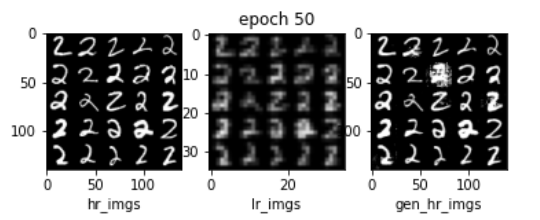
\includegraphics[width=0.46\textwidth]{figures/MNIST_all_epoch50}
    \caption{MNIST数据集 epochs = 50图像恢复结果}
    \label{MNIST_all_epoch50}
\end{figure}

如图 \ref{MNIST_all_epoch50}所示,当训练了50个epochs时,对大多数数字图像能恢复到可清晰辨识的状态,但对于少数图像的恢复效果不佳。

\begin{figure}[htp]
    \centering
    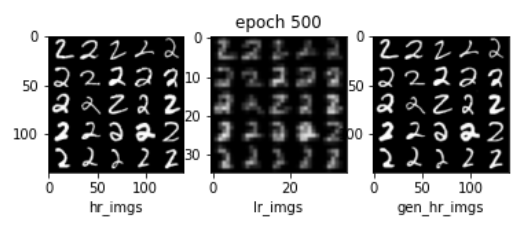
\includegraphics[width=0.46\textwidth]{figures/MNIST_all_epoch500}
    \caption{MNIST数据集 epochs = 500图像恢复结果}
    \label{MNIST_all_epoch500}
\end{figure}

\begin{figure}[htp]
    \centering
    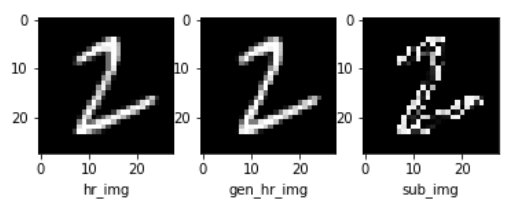
\includegraphics[width=0.46\textwidth]{figures/MNIST_sub}
    \caption{生成图像与原图的比较}
    \label{MNIST_sub}
\end{figure}

如图 \ref{MNIST_all_epoch500}、\ref{MNIST_sub}所示,当训练了1000个epochs时,模型的Loss下降到0.4以下,生成图与原图的差距较小,人眼几乎无法分辨。

\subsubsection{不同大小的图像恢复效果比较}
在对亚洲人脸数据集进行图像恢复时,我们进行了8×8图像恢复和16×16图像恢复两组实验,均只使用Condition Network进行图像恢复,并都对模型训练300epochs。

\begin{figure}[htp]
    \centering
    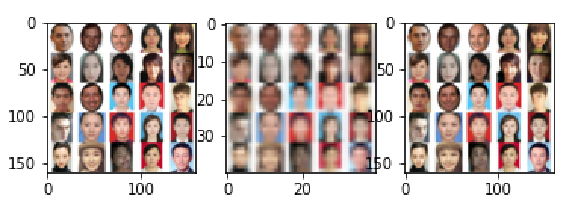
\includegraphics[width=0.46\textwidth]{figures/person_all_8}
    \caption{亚洲人脸数据集 8×8图像恢复结果}
    \label{person_all_8}
\end{figure}

\begin{figure}[htp]
    \centering
    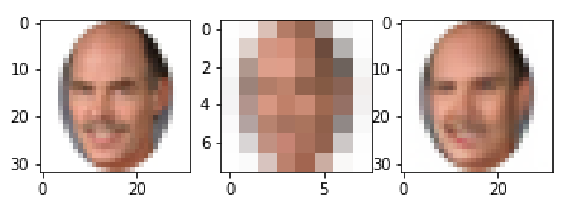
\includegraphics[width=0.46\textwidth]{figures/person_8}
    \caption{亚洲人脸数据集 8×8单张图像恢复结果}
    \label{person_8}
\end{figure}

从图\ref{person_all_8}、\ref{person_8}的图像恢复效果中我们发现,8×8的图像信息丢失严重,对于人眼来说已经很难辨识,而模型依旧能恢复出图像的大体轮廓。

\begin{figure}[htp]
    \centering
    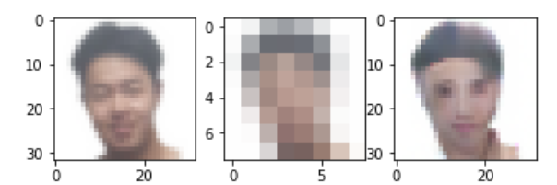
\includegraphics[width=0.46\textwidth]{figures/zzy_8}
    \caption{非正常角度的8×8图像恢复结果}
    \label{zzy_8}
\end{figure}

如图\ref{zzy_8}所示,此模型在细节上的恢复效果较差,尤其是对非正常角度拍摄的图像进行恢复时,会出现较严重的细节丢失现象,因此我们并不认为此模型在8×8这种超低分辨率的图像恢复上有较好的效果。

\begin{figure}[htp]
    \centering
    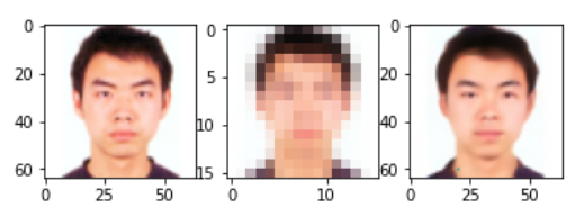
\includegraphics[width=0.46\textwidth]{figures/person_16}
    \caption{亚洲人脸数据集 16×16单张图像恢复结果}
    \label{person_16}
\end{figure}

从图\ref{person_16}中可以看出,相较于8×8图像恢复而言,16×16图像恢复在细节处理上效果更好,并且由于低分辨率图所包含的信息更大,所以图像恢复的泛化能力更强,对非正常角度的图像也有一定的回复能力。因此我们更倾向于以16×16图像恢复的效果来对我们的模型进行评价。

\subsubsection{是否使用prior network的图像恢复效果比较}
在对16×16的图像恢复的基础上,我们对Prior Network网络进行了评测,在有无Prior Network的情况下,图像恢复效果也不同。

在实验中我们发现,Condition Network与Prior Network两个网络分开训练与协同训练的图像恢复效果差别并不大。为了更公正的评测Prior Nwtwork的图像恢复效果,我们选择了两个网络分开训练的方式,以此保证了在对照实验中,Condition Network的训练效果一致,对图像恢复效果差异不造成影响。

\begin{figure}[htp]
    \centering
    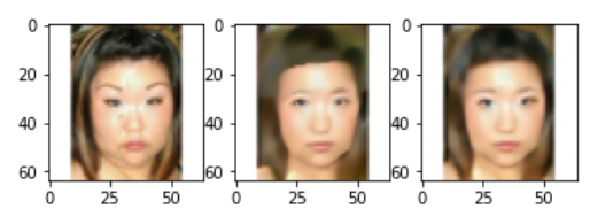
\includegraphics[width=0.46\textwidth]{figures/prior}
    \caption{是否使用Prior Network的图像恢复效果比较}
    \label{prior}
\end{figure}

如图\ref{prior}所示,相较于仅使用Condition Network的图像恢复结果而言,使用Prior Network会使得恢复出的图像在许多细节上获取到一种整体特征,比如在发型轮廓上,Prior Network会使得图像的这一部分更加真实,当然也是更接近于整体平均水平。

\subsubsection{图像恢复的局限性与泛化能力}

\begin{figure}[htp]
    \centering
    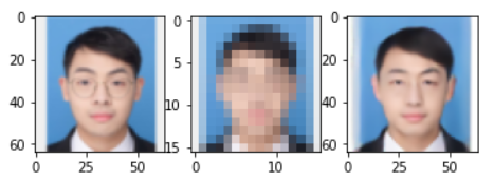
\includegraphics[width=0.46\textwidth]{figures/ly}
    \caption{戴眼镜的人物图像恢复}
    \label{ly}
\end{figure}

如图\ref{ly}所示,使用此模型进行图像恢复极其受限于数据集,当需恢复的图像包含有数据集不包含的特征(例如眼镜、胡须、辫子等)时,恢复效果会较差。

\begin{figure}[htp]
    \centering
    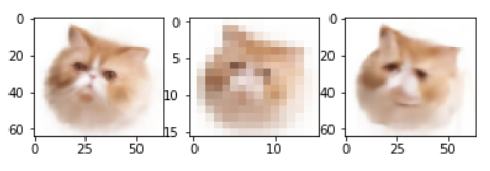
\includegraphics[width=0.46\textwidth]{figures/cat}
    \caption{非人类的人物图像恢复}
    \label{cat}
\end{figure}

如图\ref{cat}所示,当对非人类图像进行预测时该模型也有一定的预测效果,一方面说明模型并未过拟合,另一方面说明该模型具有一定的泛化能力,能够较为准确地提供一种对各类图像的恢复方案。

\subsection{图像相似性的定量评估}
对图像相似性的量化方法有很多,最常见的有均方误差MSE, 结构相似性SSIM, 以及峰值信噪比PSNR三种,我们在实验中使用到的图像相似性量化标准为均方误差MSE。

\begin{figure}[htp]
    \centering
    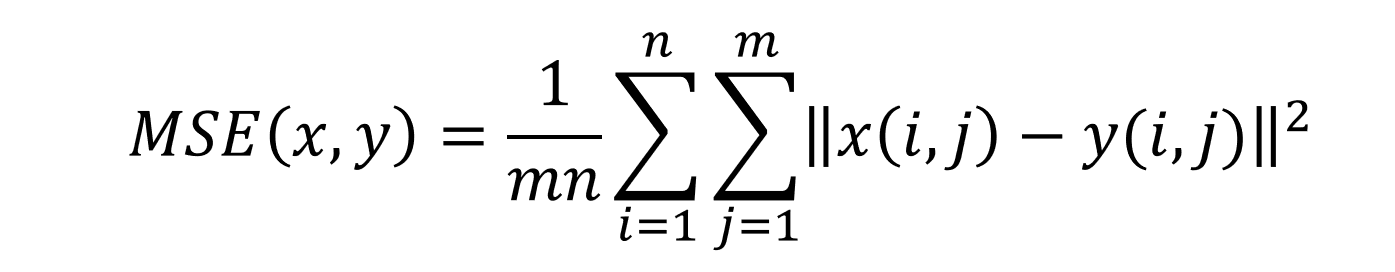
\includegraphics[width=0.46\textwidth]{figures/mse}
    \caption{均方误差MSE}
\end{figure}

\subsection{对人类的感知评估}
在误差分析过程中我们发现,定量的方式实际上与人类的感知判断并不完全相符,很多看起来恢复效果不佳的图像却定量评估上表现较好。因此在后续的调节过程与最终的模型效果评判上,我们更多地参考了人类的感知来对模型进行调整与评价。
